\documentclass{article}

\usepackage{amsmath}
\usepackage{amssymb}
\usepackage{graphicx}

\begin{document}


Ivan Lin\newline{}
Dr. Esther Arkin\newline{}
AMS301\newline{}
2/17/17

\begin{center}
  Homework 4a
\end{center}

\underline{Section 2.3 Question 1 Part K}

The chromatic color for the graph is 2. Every edge between two vertices is a $K_2$ subgraph. Therefore there must be at least two colors to prevent adjacent nodes from sharing a color.

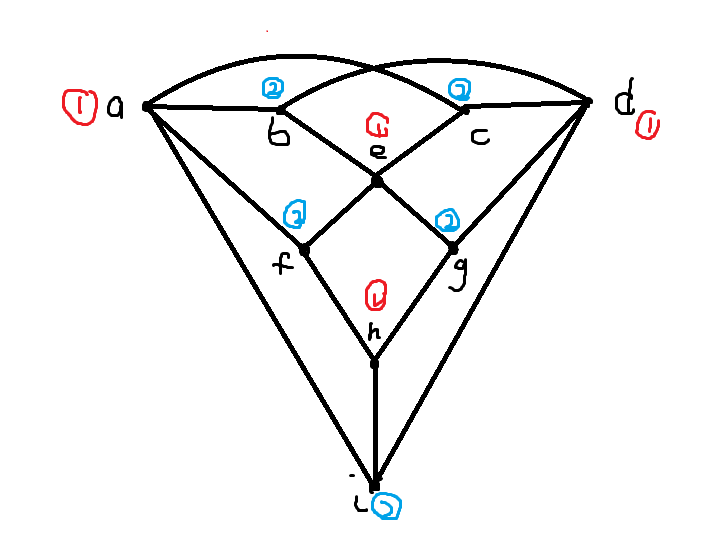
\includegraphics[height=100px]{hw3-1k.png}

\underline{Section 2.3 Question 1 Part O}

The chromatic color for the graph is 4. The largest complete subgraph of the graph is $K_3$, so we can try and build 3-color the graph. Start coloring the triangle $b-a-c$ with colors $1-2-3$ respectively. Vertex $d$ is adjacent to both $a$ and $c$, so it must be the same color as $b$. Vertex $i$ is adjacent to $b$ and $c$ while vertex $j$ is adjacent to $c$ and $d$, so they must both be colored the same as vertex $a$. However, this is not possible, since vertices $i$ and $j$ are connected to each other. The graph therefore can not be three colored. A four colored configuration si possible.

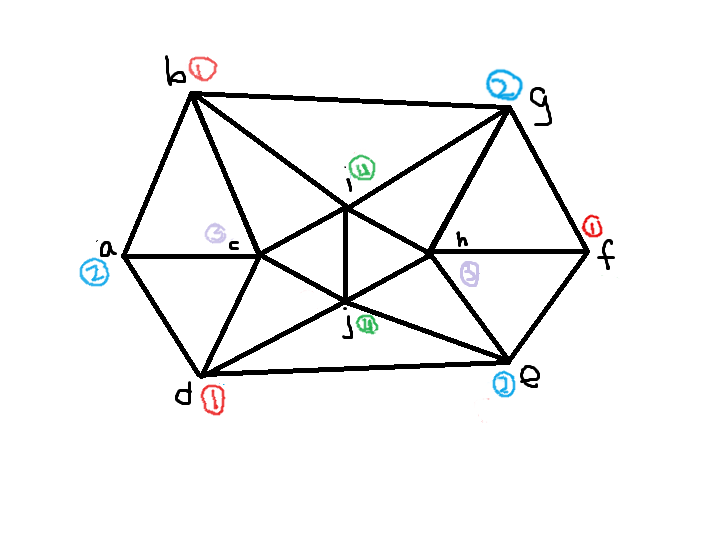
\includegraphics[height=100px]{hw3-1o.png}

\underline{Section 2.3 Question 2 Part A}

All vertices have a degree of 3, meaning the graph's edges cannot be any less than three colored.

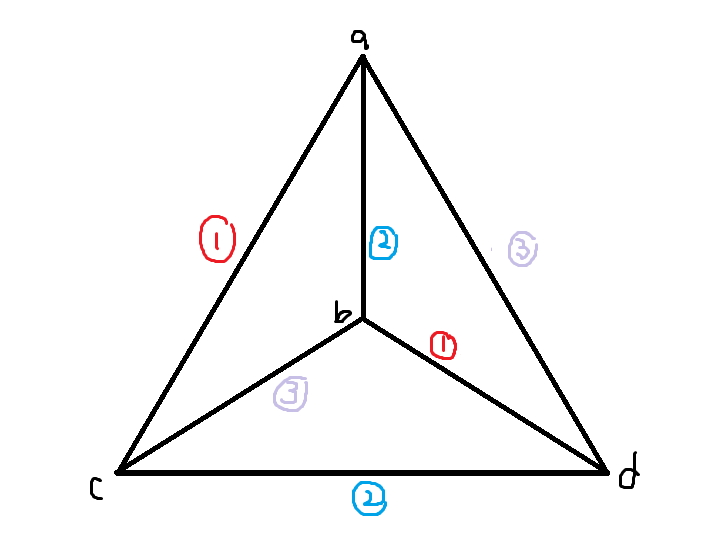
\includegraphics[height=100px]{hw3-2a.png}

\underline{Section 2.3 Question 2 Part B}

All vertices have a degree of 3, meaning the graph's edges cannot be any less than three colored.

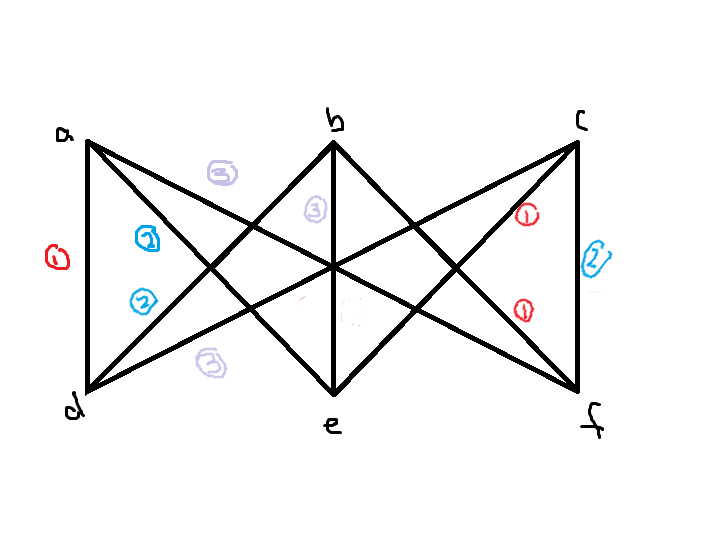
\includegraphics[height=100px]{hw3-2b.png}

\end{document}
